
\begin{figure}[H]
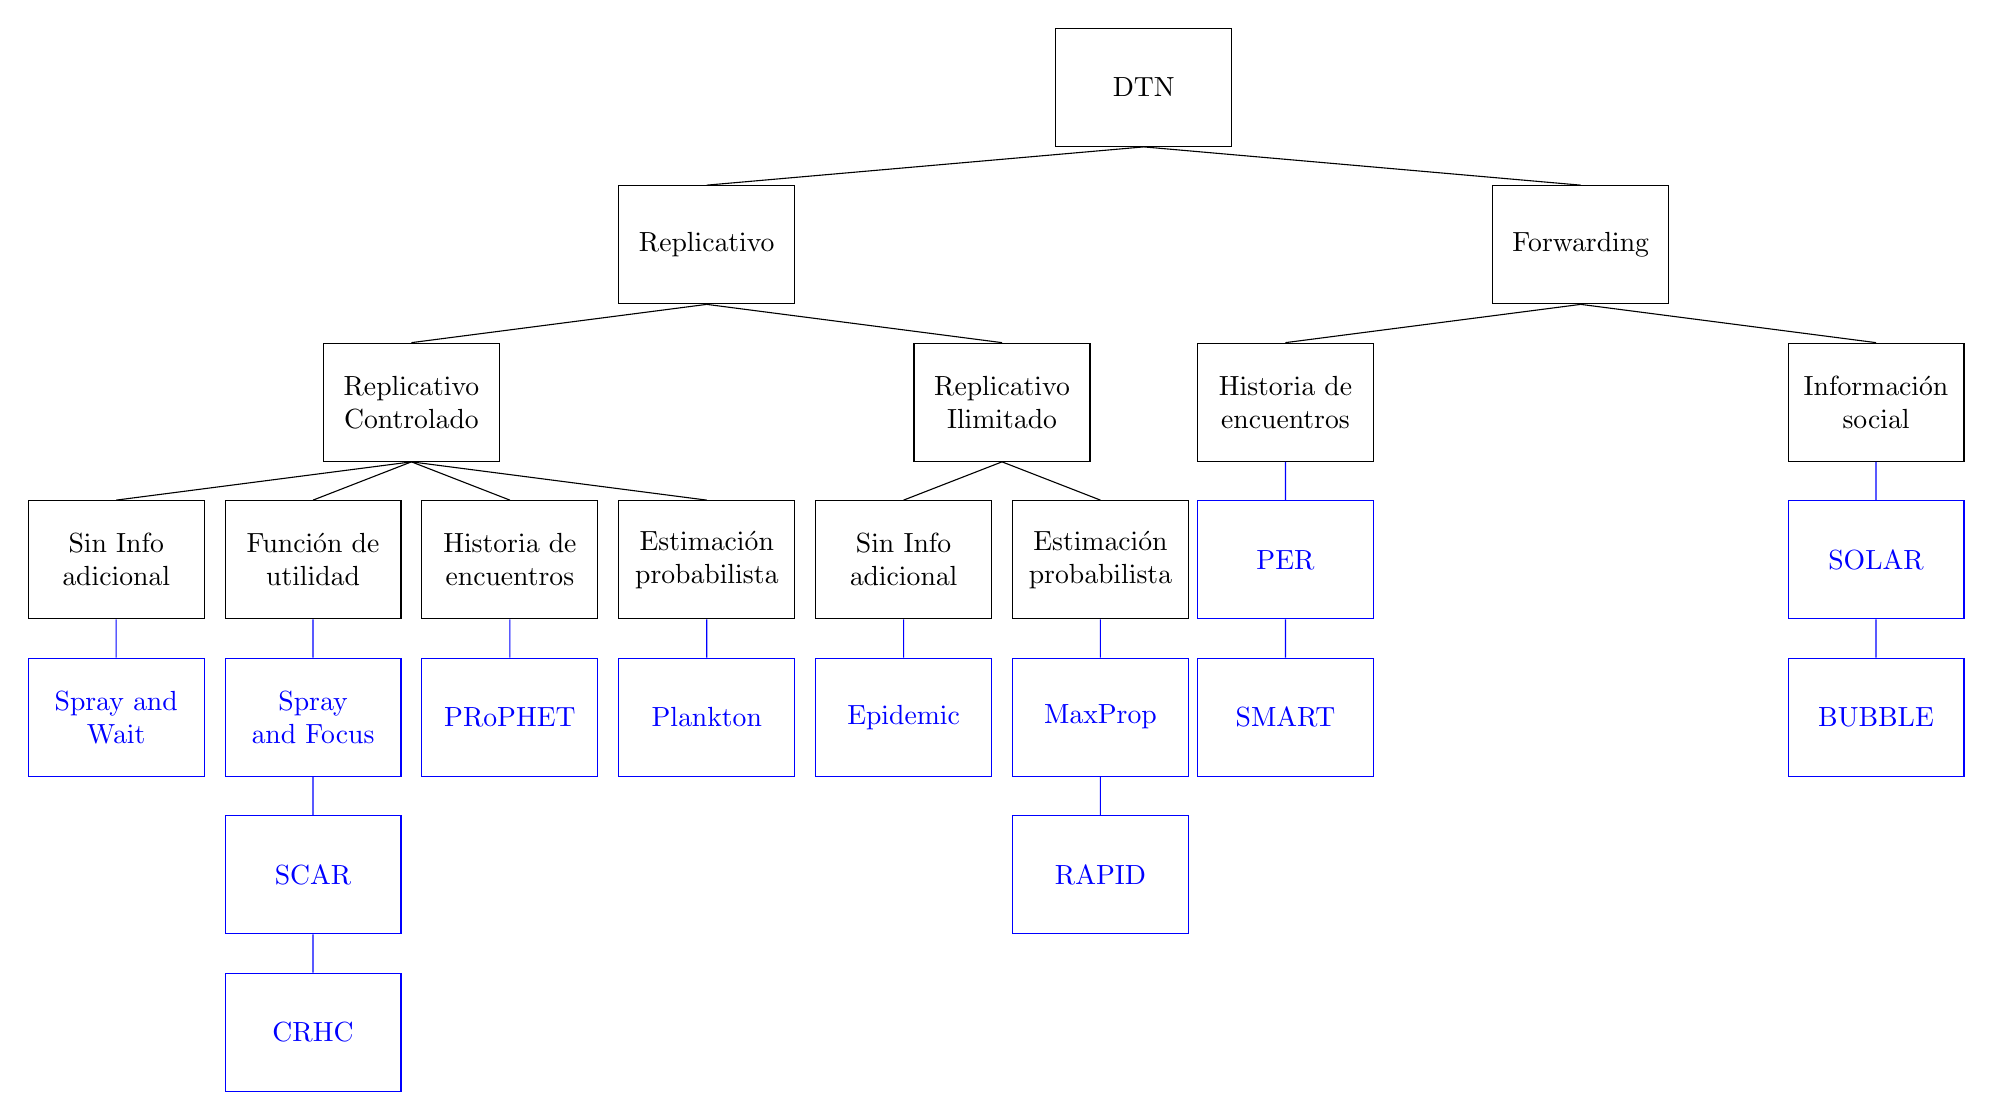
\begin{tikzpicture}
  [auto,every node/.style={rectangle,draw, text centered, text width=2.0cm,minimum height=1.5cm },node distance=4cm]
\tikzset{%
level 1/.style={sibling distance = 11.1cm, level distance=2cm,edge from parent path={(\tikzparentnode.south) -- (\tikzchildnode.north)}},
level 2/.style={sibling distance = 7.5cm, level distance=2cm,edge from parent path={(\tikzparentnode.south) -- (\tikzchildnode.north)}},
level 3/.style={sibling distance = 2.5cm, level distance=2cm,edge from parent path={(\tikzparentnode.south) -- (\tikzchildnode.north)}},
level 4/.style={sibling distance = 2.5cm, level distance=2cm,edge from parent path={(\tikzparentnode.south) -- (\tikzchildnode.north)}},
level 5/.style={sibling distance = 2.5cm, level distance=2cm,edge from parent path={(\tikzparentnode.south) -- (\tikzchildnode.north)}},
level 6/.style={sibling distance = 2.5cm, level distance=2cm,edge from parent path={(\tikzparentnode.south) -- (\tikzchildnode.north)}},
}

\node (0){DTN}
    child {node (1) {Replicativo}
              child {node (2) {Replicativo \\Controlado}
                child{node (3) {Sin Info \\ adicional}
                    child[blue]{node (4) {Spray and \\Wait}}}
                child{node {Función de \\ utilidad}
                    child[blue]{node {Spray and Focus}
                    child{node {SCAR}
                    child{node {CRHC}}}}}
                child{node {Historia de \\ encuentros}
                    child[blue]{node{PRoPHET}}}
                child{node {Estimación \\ probabilista}
                    child[blue]{node{Plankton}}}}
              child {node {Replicativo \\Ilimitado}
                child{node {Sin Info \\ adicional}
                    child[blue]{node {Epidemic}}}
                child{node {Estimación \\ probabilista}
                    child[blue]{node {MaxProp}
                    child{node {RAPID}}}}}
              }
    child {node {Forwarding}
              child {node (5){Historia de \\ encuentros}
                child[blue] {node (6){PER}
                child {node {SMART}}}}
              child {node (5){Información \\ social}
                child[blue] {node (6){SOLAR}
                child {node {BUBBLE}}}}};
\end{tikzpicture}

\end{figure}
